\documentclass[11pt]{article}
\usepackage[margin=1in]{geometry}

\usepackage{amsmath}
\usepackage{amssymb}
\usepackage[utf8]{inputenc} 
\usepackage{graphicx} 
\usepackage{parskip} 
\usepackage{multirow} 
\usepackage{mathtools}

\DeclarePairedDelimiter\abs{\lvert}{\rvert}%
\DeclarePairedDelimiter\norm{\lVert}{\rVert}%

\makeatletter
\let\oldabs\abs
\def\abs{\@ifstar{\oldabs}{\oldabs*}}

\let\oldnorm\norm
\def\norm{\@ifstar{\oldnorm}{\oldnorm*}}
\makeatother
\usepackage{multicol} 
\usepackage[spanish,es-nodecimaldot]{babel} 
\usepackage{mathtools}
\usepackage{amsfonts}
\usepackage{float}
\usepackage{textcomp}
\usepackage{caption}
\usepackage{subfig}
\usepackage[spanish]{babel}
\usepackage{gensymb}
\def\sen{\mathop{\mbox{\normalfont sen}}\nolimits}

\usepackage{fancyhdr}
\fancyhf{}
\rfoot{\thepage}
\pagestyle{fancy}
\lhead{Nieto Castellanos Jaime Fabián}
\chead{}
\rhead{Tarea 6. Histogramas}
\begin{document}

\textbf{Problema 1}
\begin{figure}[H]
\centering
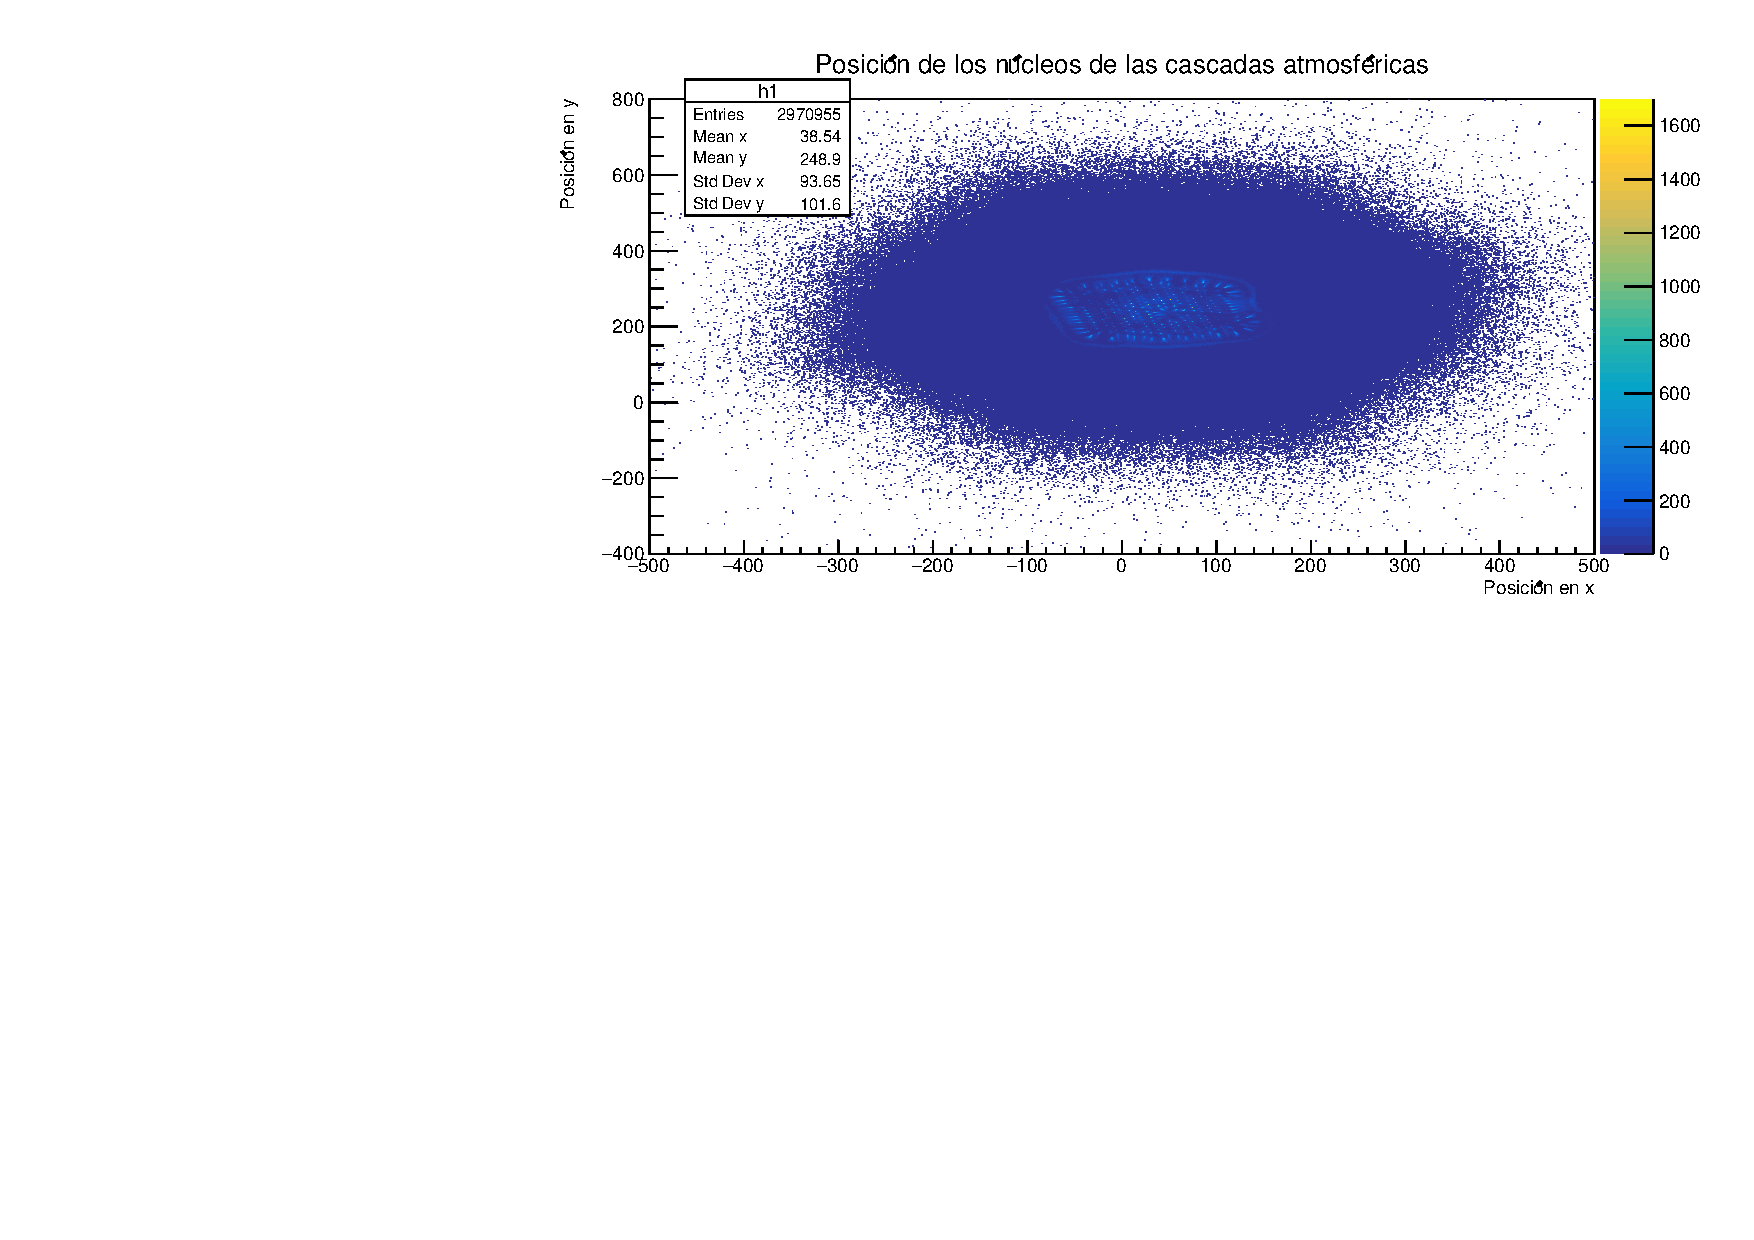
\includegraphics[width=1 \textwidth]{../Figuras/Prob1}
\caption{Histogramas bidimensional que muestra las posiciones de los núcleos de las cascadas atmosféricas. Se hizo un corte de selección.}
\label{fig:Prob1}
\end{figure}
\textbf{Problema 2}
\begin{figure}[H]
\centering
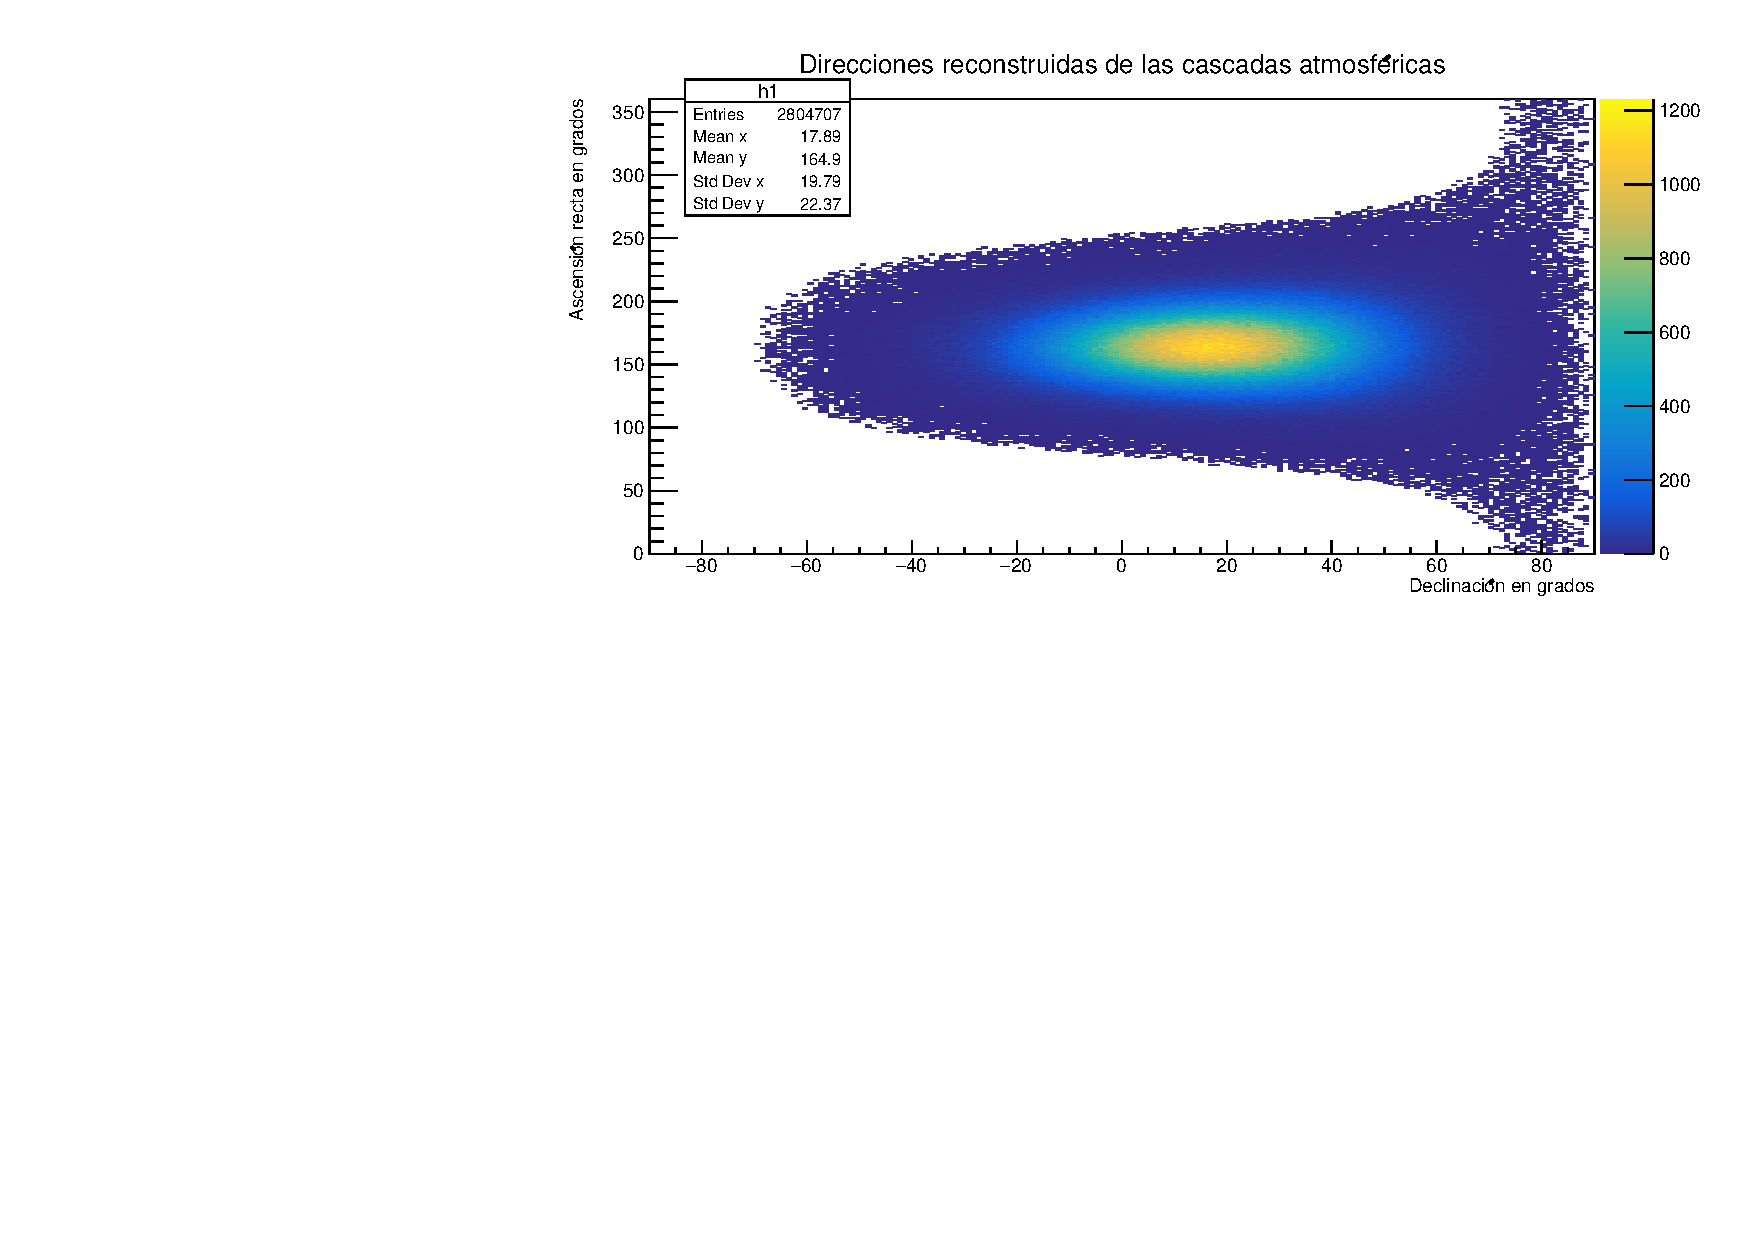
\includegraphics[width=1 \textwidth]{../Figuras/Prob2}
\caption{Histogramas bidimensional que muestra las direcciones, en coordenadas celestes, de los núcleos de las cascadas atmosféricas. Se hizo un corte de selección.}
\label{fig:Prob2}
\end{figure}

\pagebreak

\textbf{Problema 3}
\begin{figure}[H]
\centering

\subfloat[Distribución del número de hits a 10 ns]{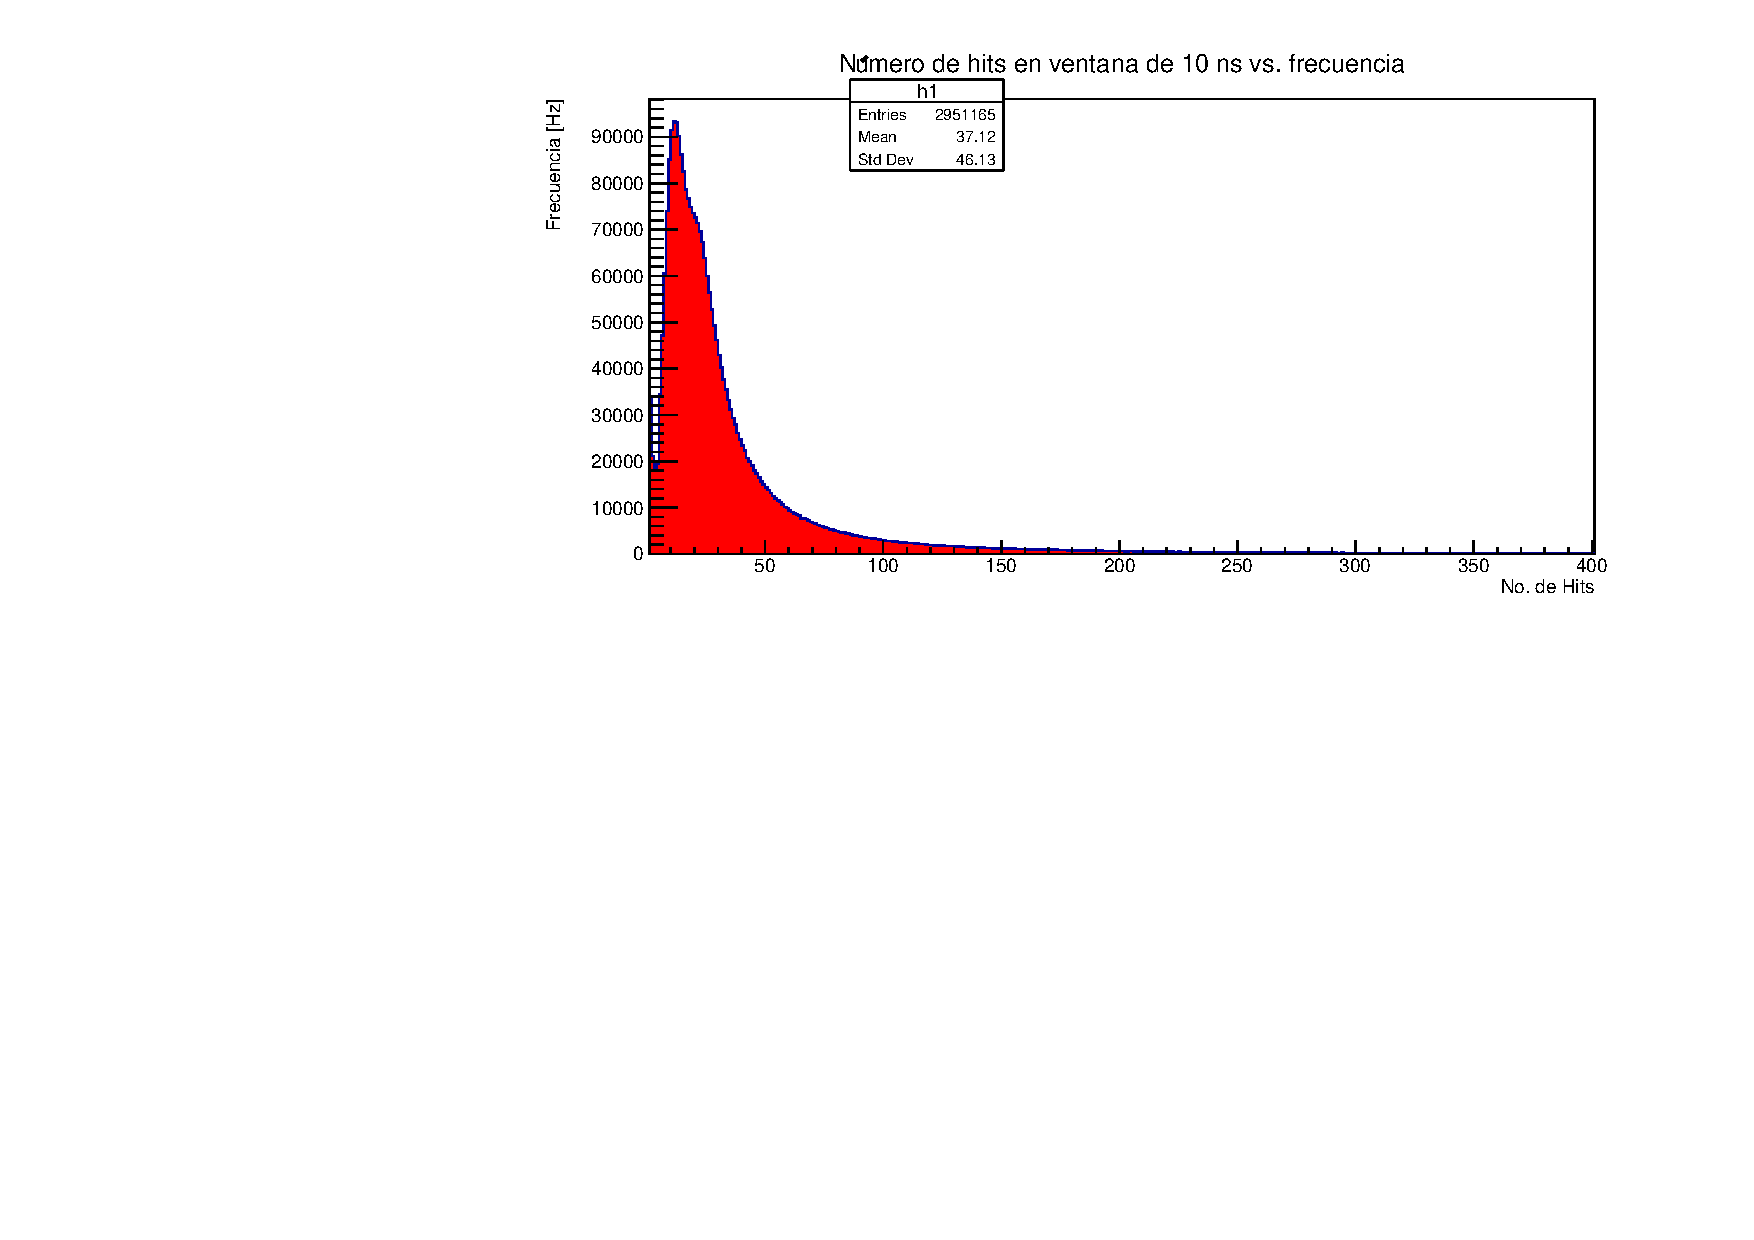
\includegraphics[width=1\textwidth]{../Figuras/Prob310Ns}}

\subfloat[Distribución del número de hits a 20 ns]{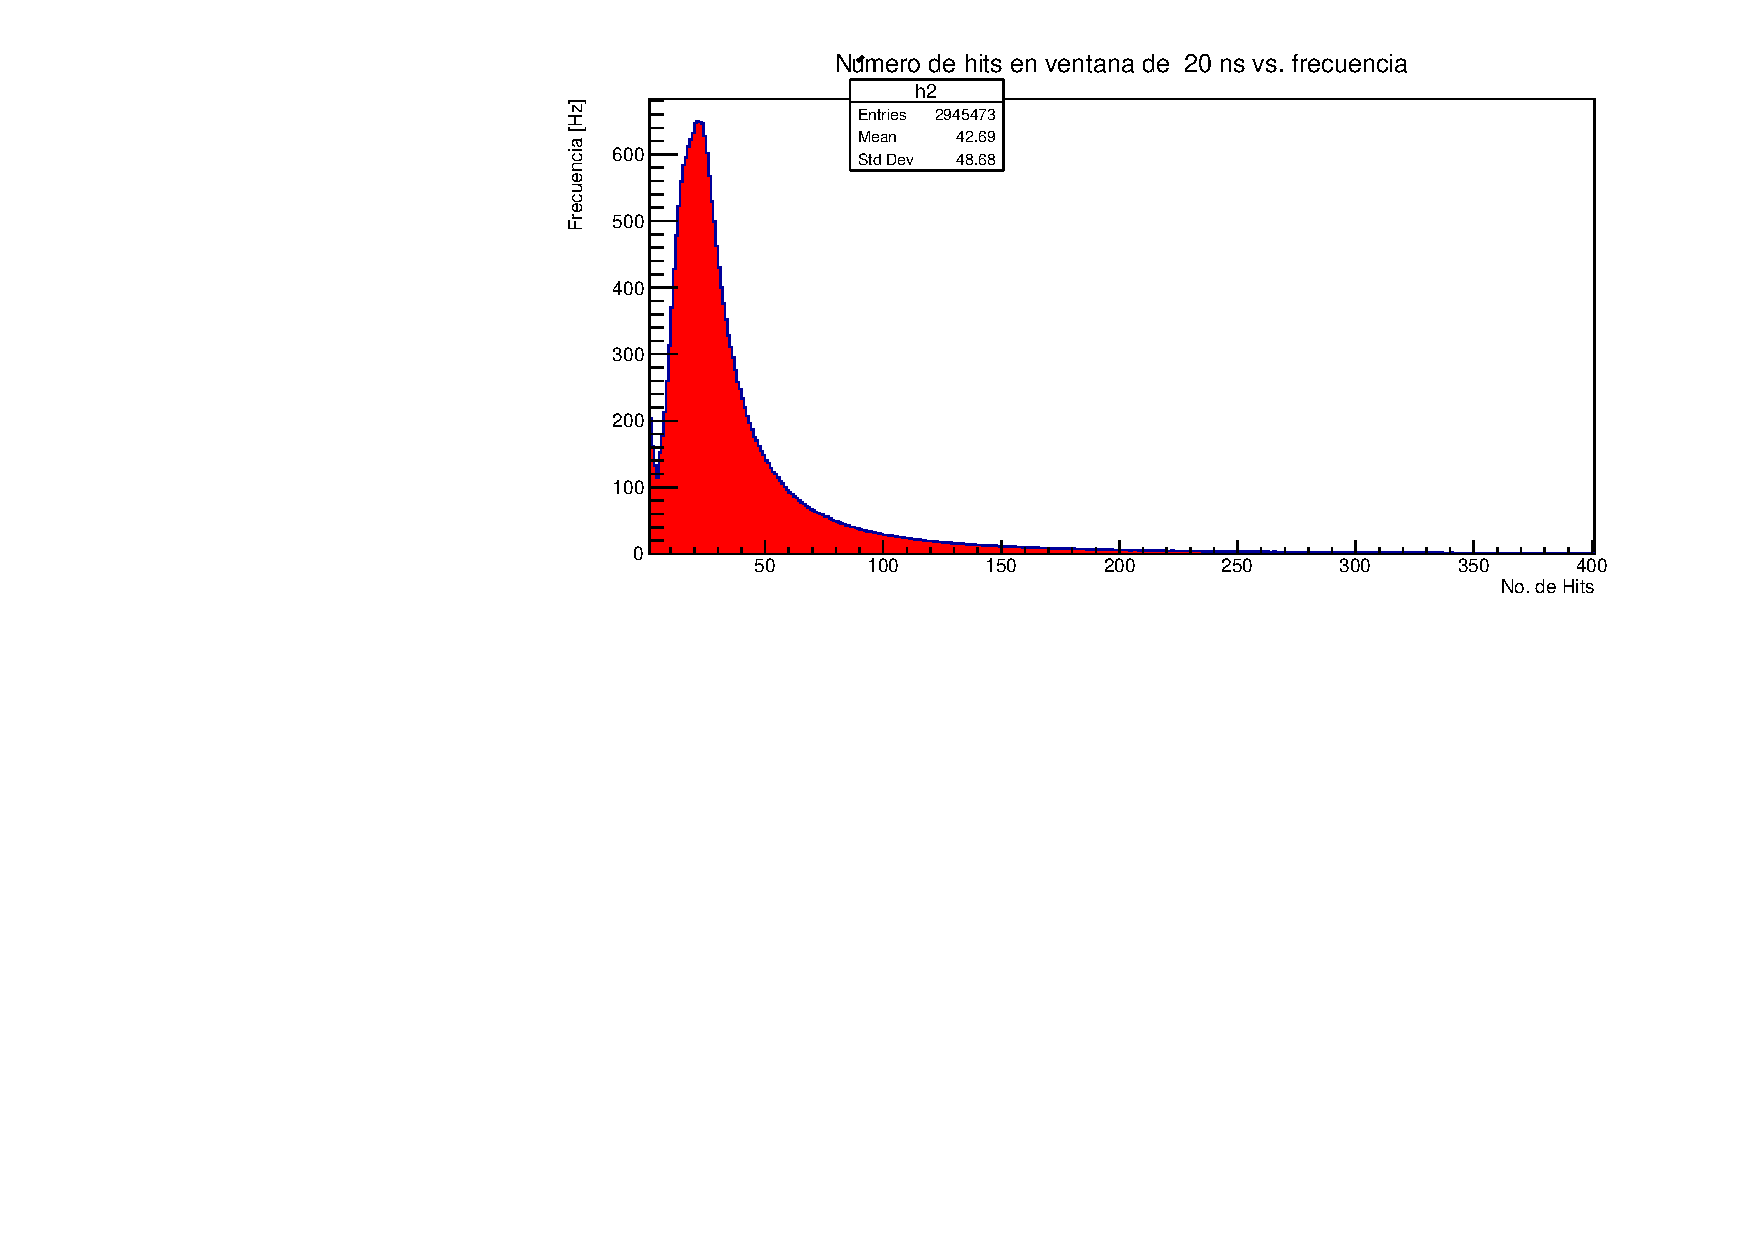
\includegraphics[width=1\textwidth]{../Figuras/Prob320Ns}}
\caption{Distribución del número de hits de todos los eventos.}
\end{figure}

\textbf{A) ¿Con qué frecuencia [Hz] se detectan cascadas con >100 hits a 10 ns del frente de la cascada?}
La respuesta de cómo se obtiene el resultado la pueden encontrar en el archivo que se llama Prob3.C, aquí solo pongo el resultado: 1698.5 Hz.

\textbf{B) ¿Con qué frecuencia [Hz] se detectan cascadas con >500 hits a 20 ns del frente de la cascada?}
116.72 Hz.
\pagebreak

\textbf{Problema 4}
\textbf{a)}
\begin{figure}[H]
\centering
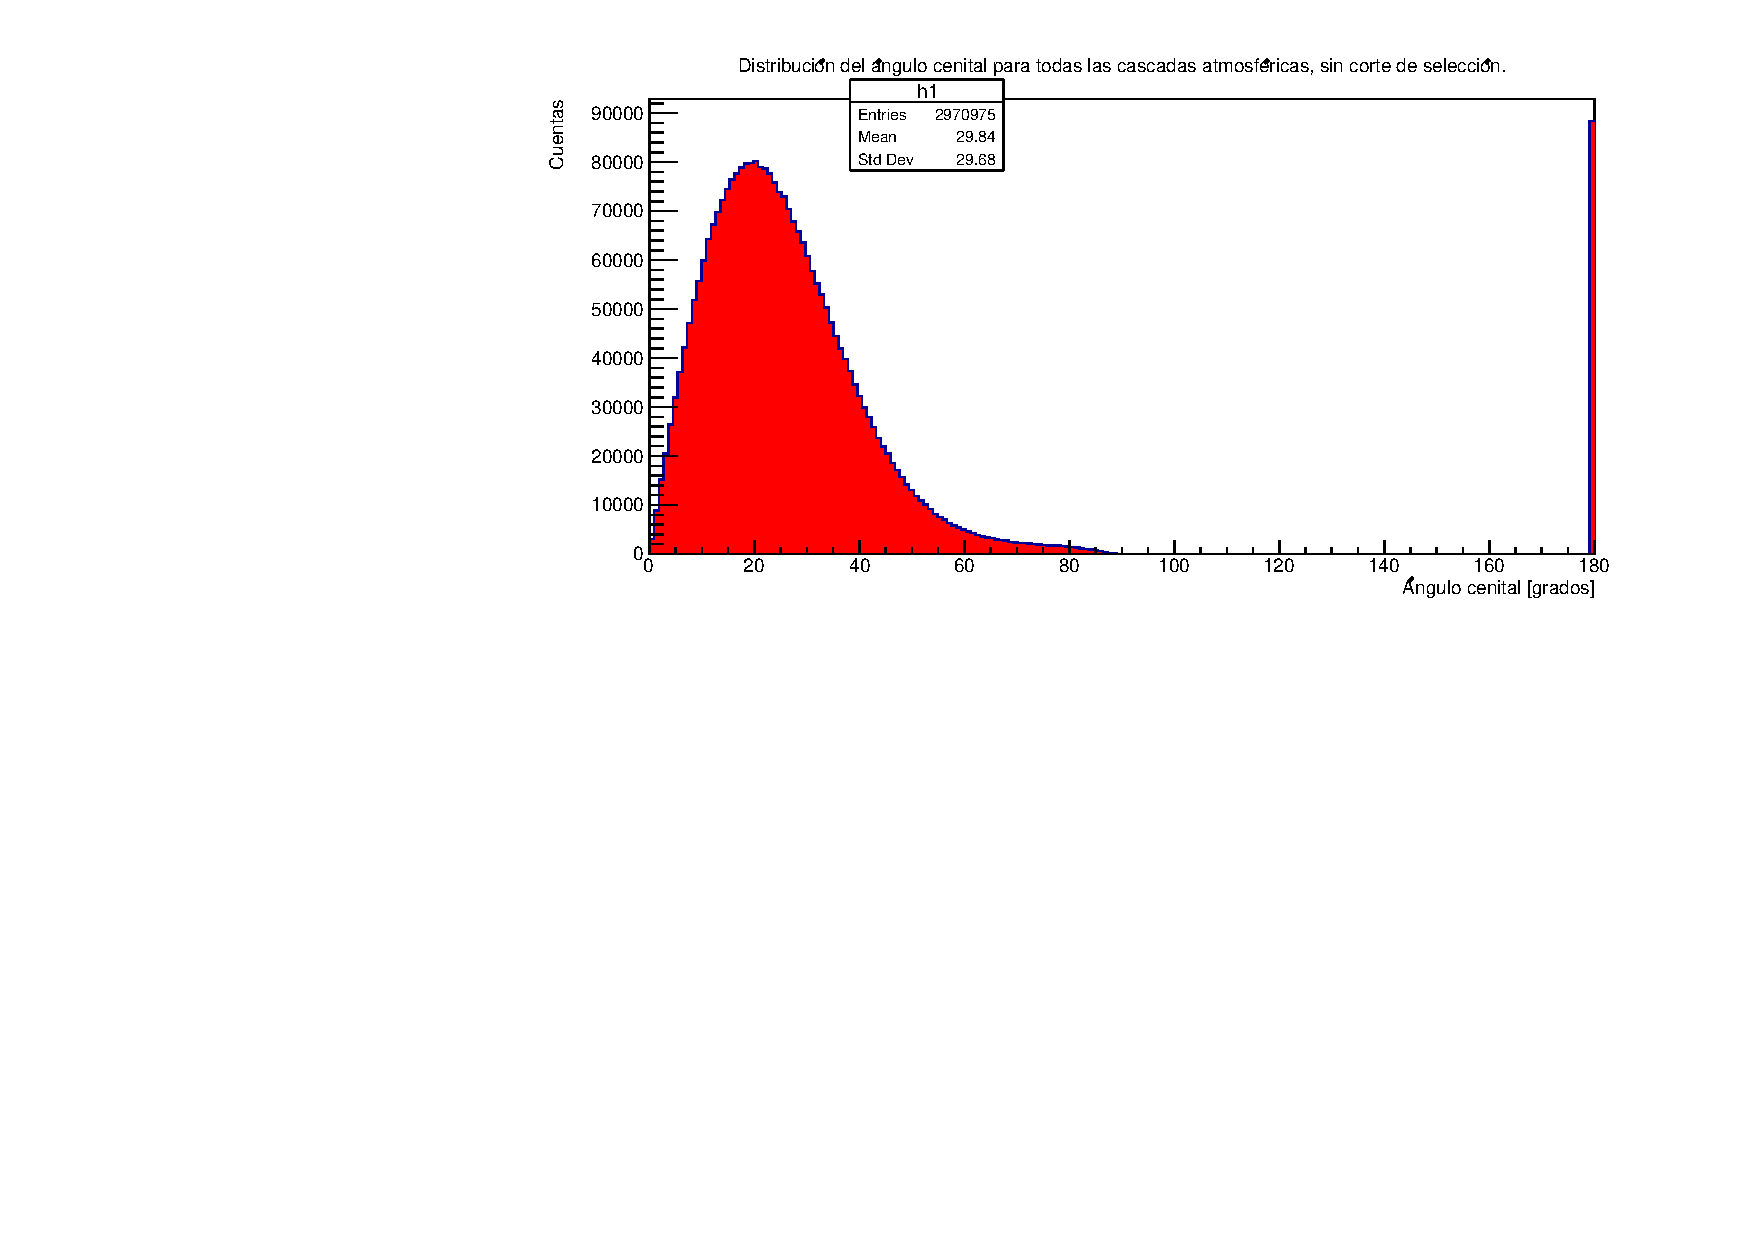
\includegraphics[width=1\textwidth]{../Figuras/Prob4A}
\caption{Distribución del ángulo cenital para todos los eventos sin corte de selección}
\label{fig:Prob4A}
\end{figure}
En la figura \ref{fig:Prob4A} se observa que hay un pico muy grande cercano a 180°, lo cual resulta extraño. Sin embargo, lo más posible es que ese pico sea un problema al momento de reconstruir el ángulo cenital, ya que al hacer el corte de calidad (figura \ref{fig:Prob4B}) el pico ya no se observa. La fracción total de eventos que pasan por el corte de selección la determinamos contando el número de eventos para los cuales la variable angleFitSatus es cero y dividiendo sobre el número total de eventos, se obtiene 0.944, es decir, el 94.4\% de los eventos tienen una buena reconstrucción angular. Como esta variable es la misma para el ángulo cenital como el azimutal, la fracción es la misma en ambos casos.

Ahora bien, para analizar el área que barren los bines del histograma, lo que se puede hacer es considerar primero una esfera de radio 1. Lo que haremos será graficar los cortes horizontales de esa esfera correspondientes a los valores extremos de un bin del ángulo cenital. Es decir, supongamos que tenemos $n$ bines, entonces cada bin tiene una longitud $\pi/n$, por lo que los valores extremos del primer bin son $0,\pi/n$, los del segundo bin son $\pi/n, 2\pi/n$, los del tercero $2\pi/n, 3\pi/n$ y así sucesivamente. Graficaremos círculos de radio $\sin(\theta)$, donde $\theta$ corresponde a los valores extremos de los bines, y veremos que el área entre esos círculos no es constante, sino que incrementa y eventualmente disminuye. Es decir, el área barrida por cada bin no es igual. Consideramos un caso sencillo con 10 bines, debido a que si usamos un número muy grande, los círculos concéntricos estarán muy juntos y no se podrá distinguir bien el efecto. El resultado se muestra en la figura \ref{fig:Circulo}.

\begin{figure}[H]
\centering
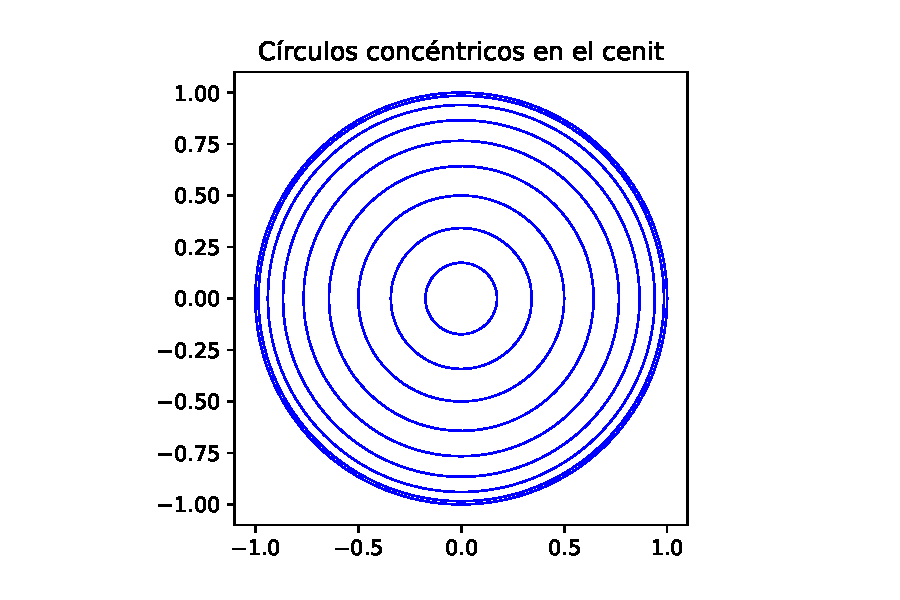
\includegraphics[width=1\textwidth]{../Figuras/Prob4Circ}
\caption{El área entre los círculos corresponde al área que barre cada uno de los bines. En el centro se encuentra el cenit. Se observa que el área no es constante}
\label{fig:Circulo}
\end{figure}
\textbf{b)}
\begin{figure}[H]
\centering
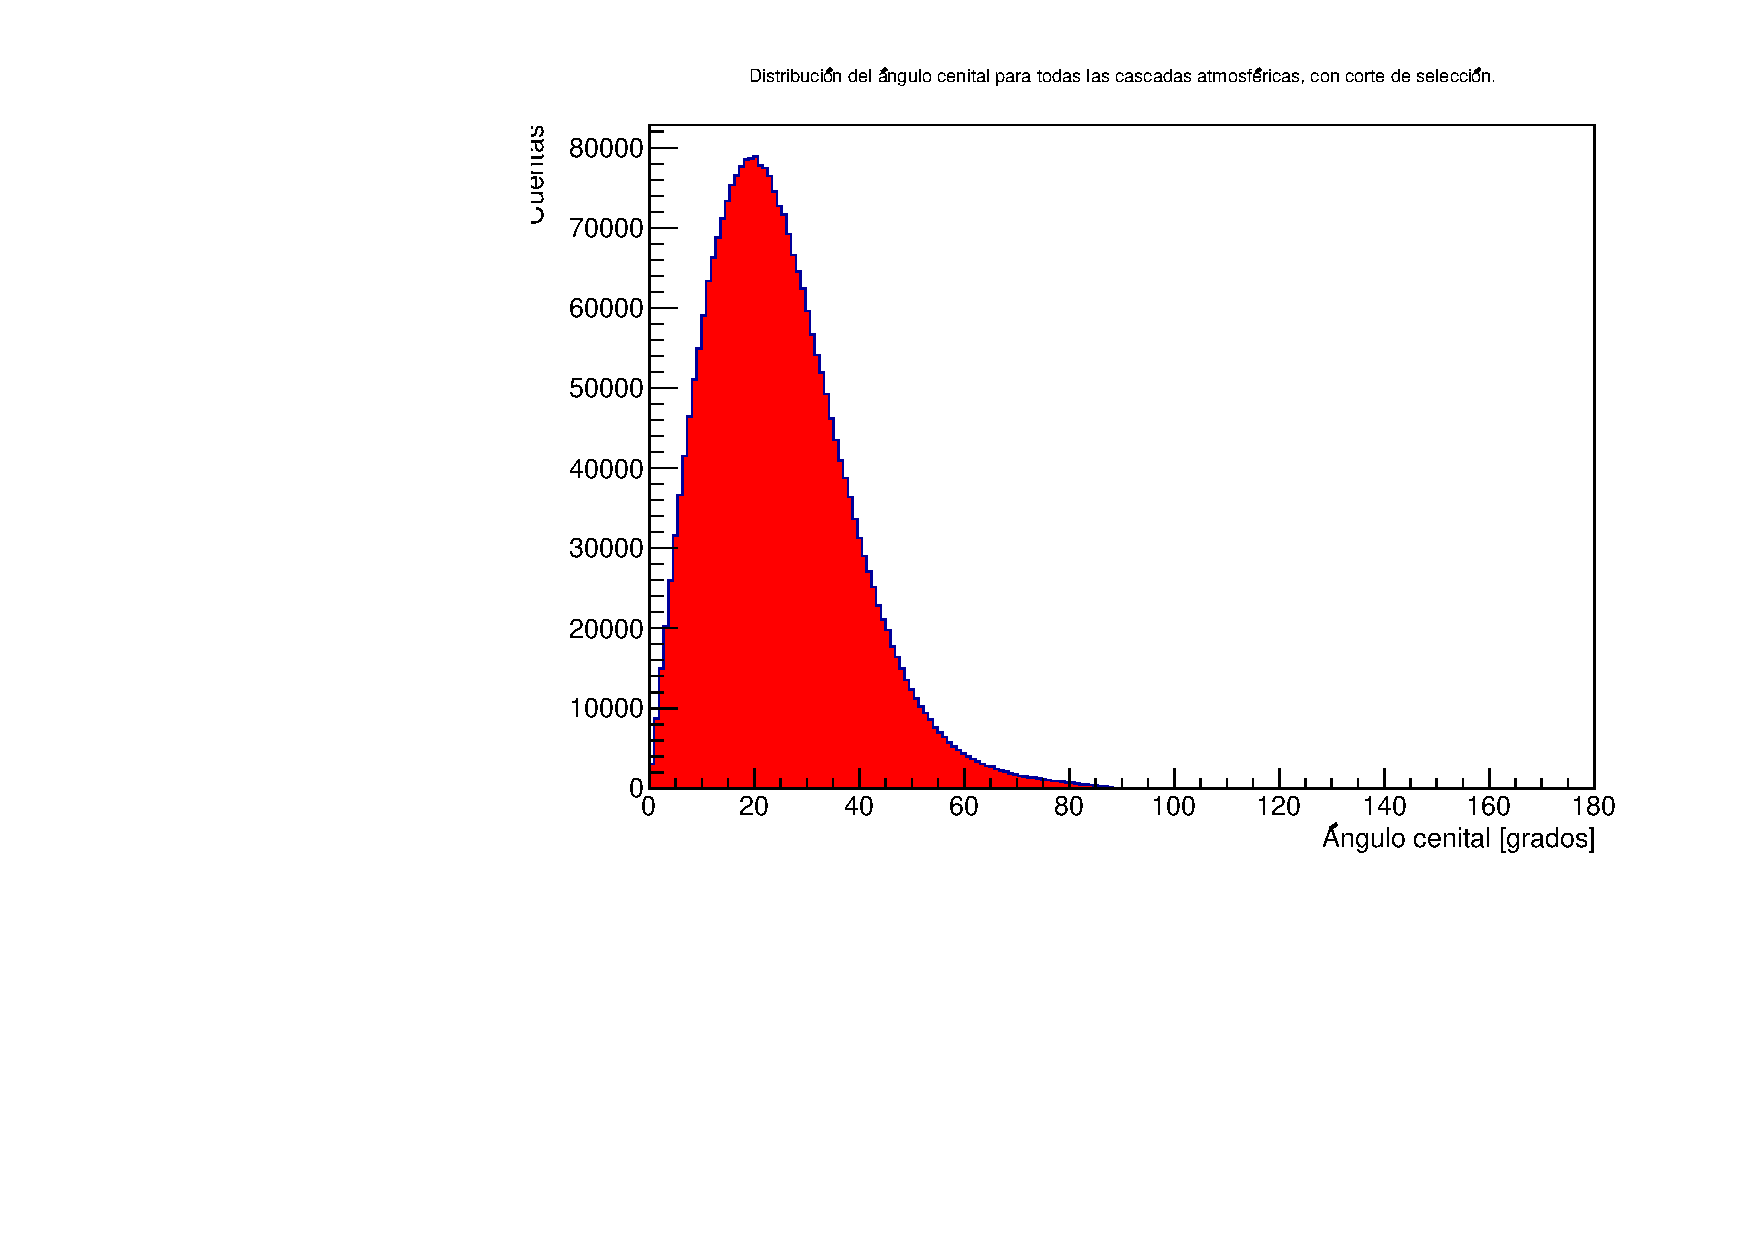
\includegraphics[width=1\textwidth]{../Figuras/Prob4B}
\caption{Distribución del ángulo cenital para todos los eventos con corte de selección}
\label{fig:Prob4B}
\end{figure}
\pagebreak

\textbf{Problema 5}
\textbf{a)}
\begin{figure}[H]
\centering
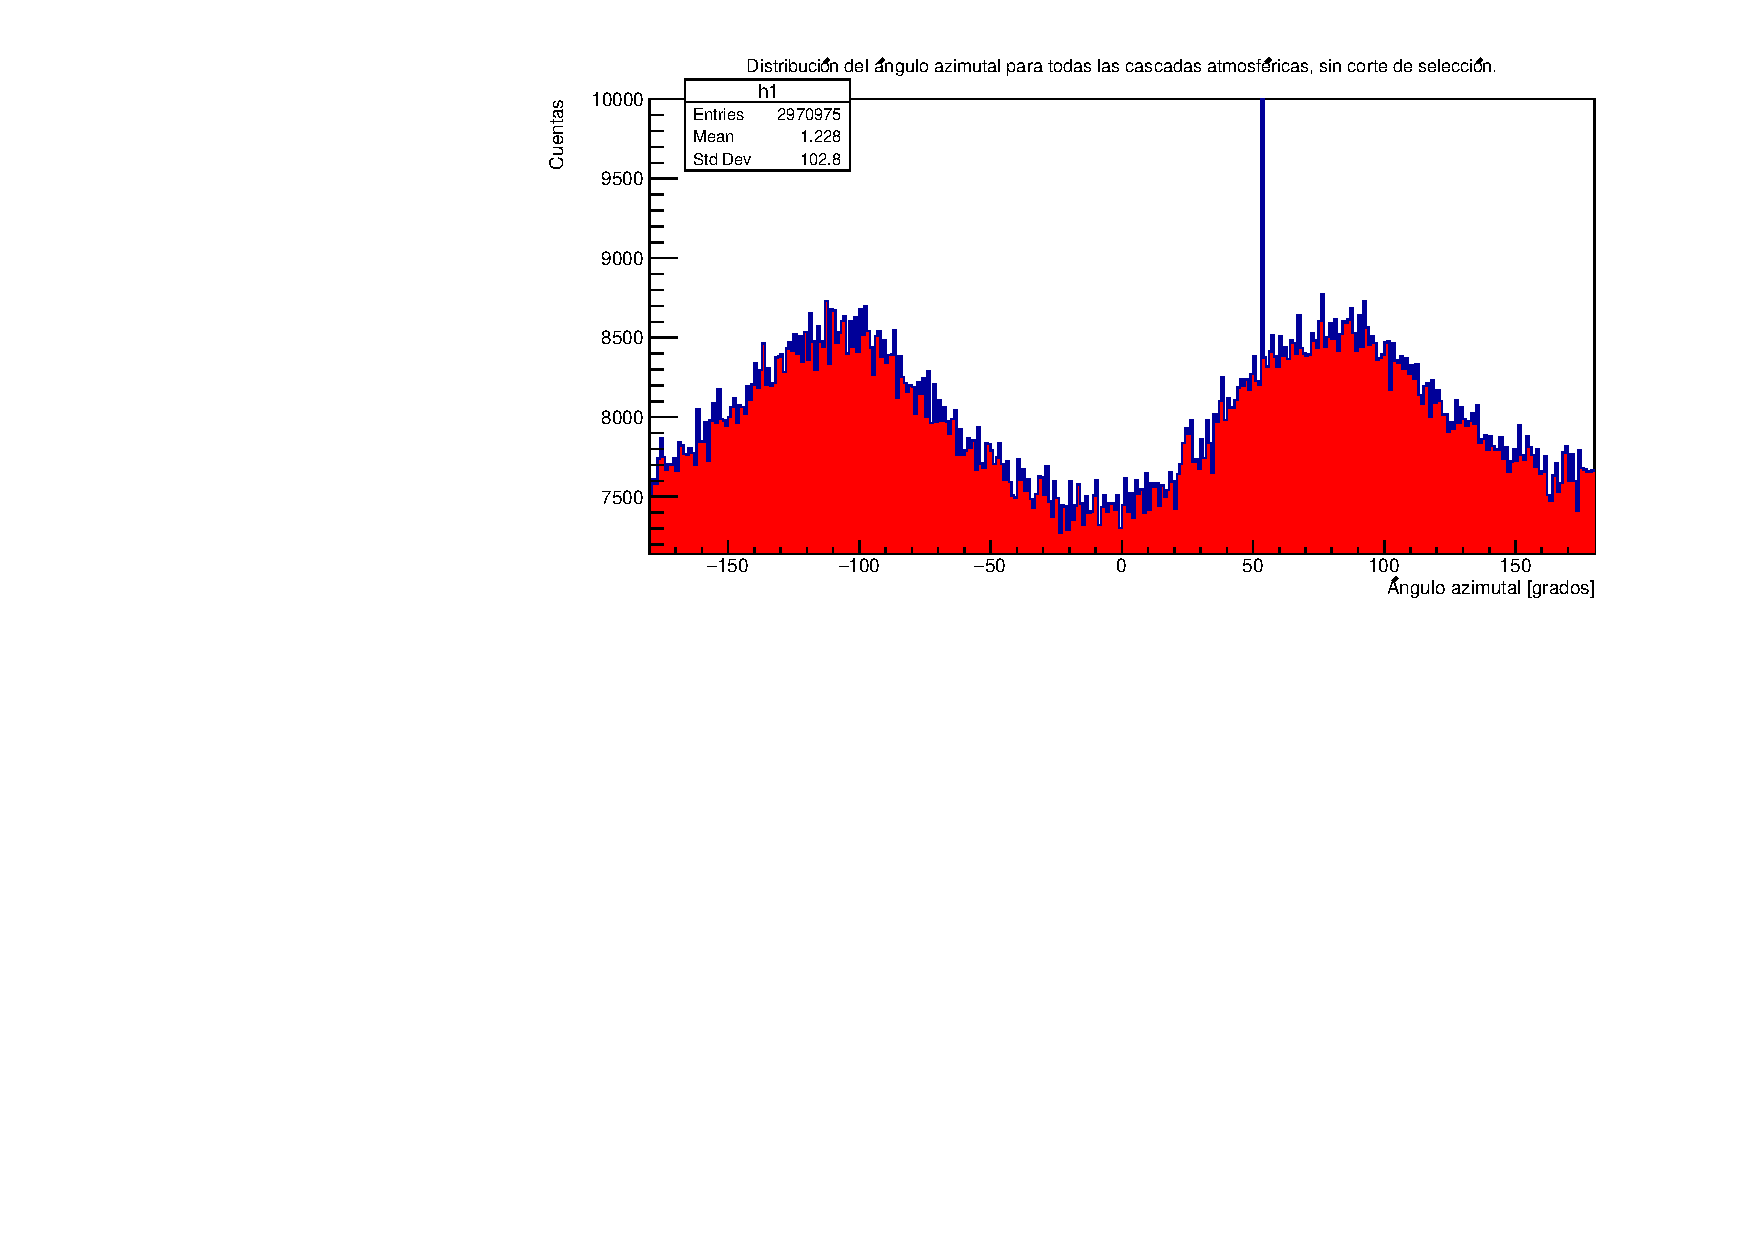
\includegraphics[width=1\textwidth]{../Figuras/Prob5A}
\caption{Distribución del ángulo azimutal para todos los eventos sin corte de selección}
\label{fig:Prob5A}
\end{figure}
En la figura \ref{fig:Prob5A} se observa que hay un pico muy grande cercano a 60°. Nuevamente, lo más posible es que ese pico sea un problema al momento de reconstruir el ángulo azimutal, ya que al hacer el corte de calidad (figura \ref{fig:Prob4B}) el pico ya no se observa. Además, la distribución es simétrica en vez de ser uniforme como uno esperaría, pues en principio podrían llegar cascadas atmosféricas desde cualquier dirección. No obstante, el campo magnético de la Tierra puede alterar las trayectorias de alguna partículas, haciendo que haya direcciones aparentemente preferenciales. La fracción total de eventos que pasan el corte de selección es 0.944. 

\textbf{b)}
\begin{figure}[H]
\centering
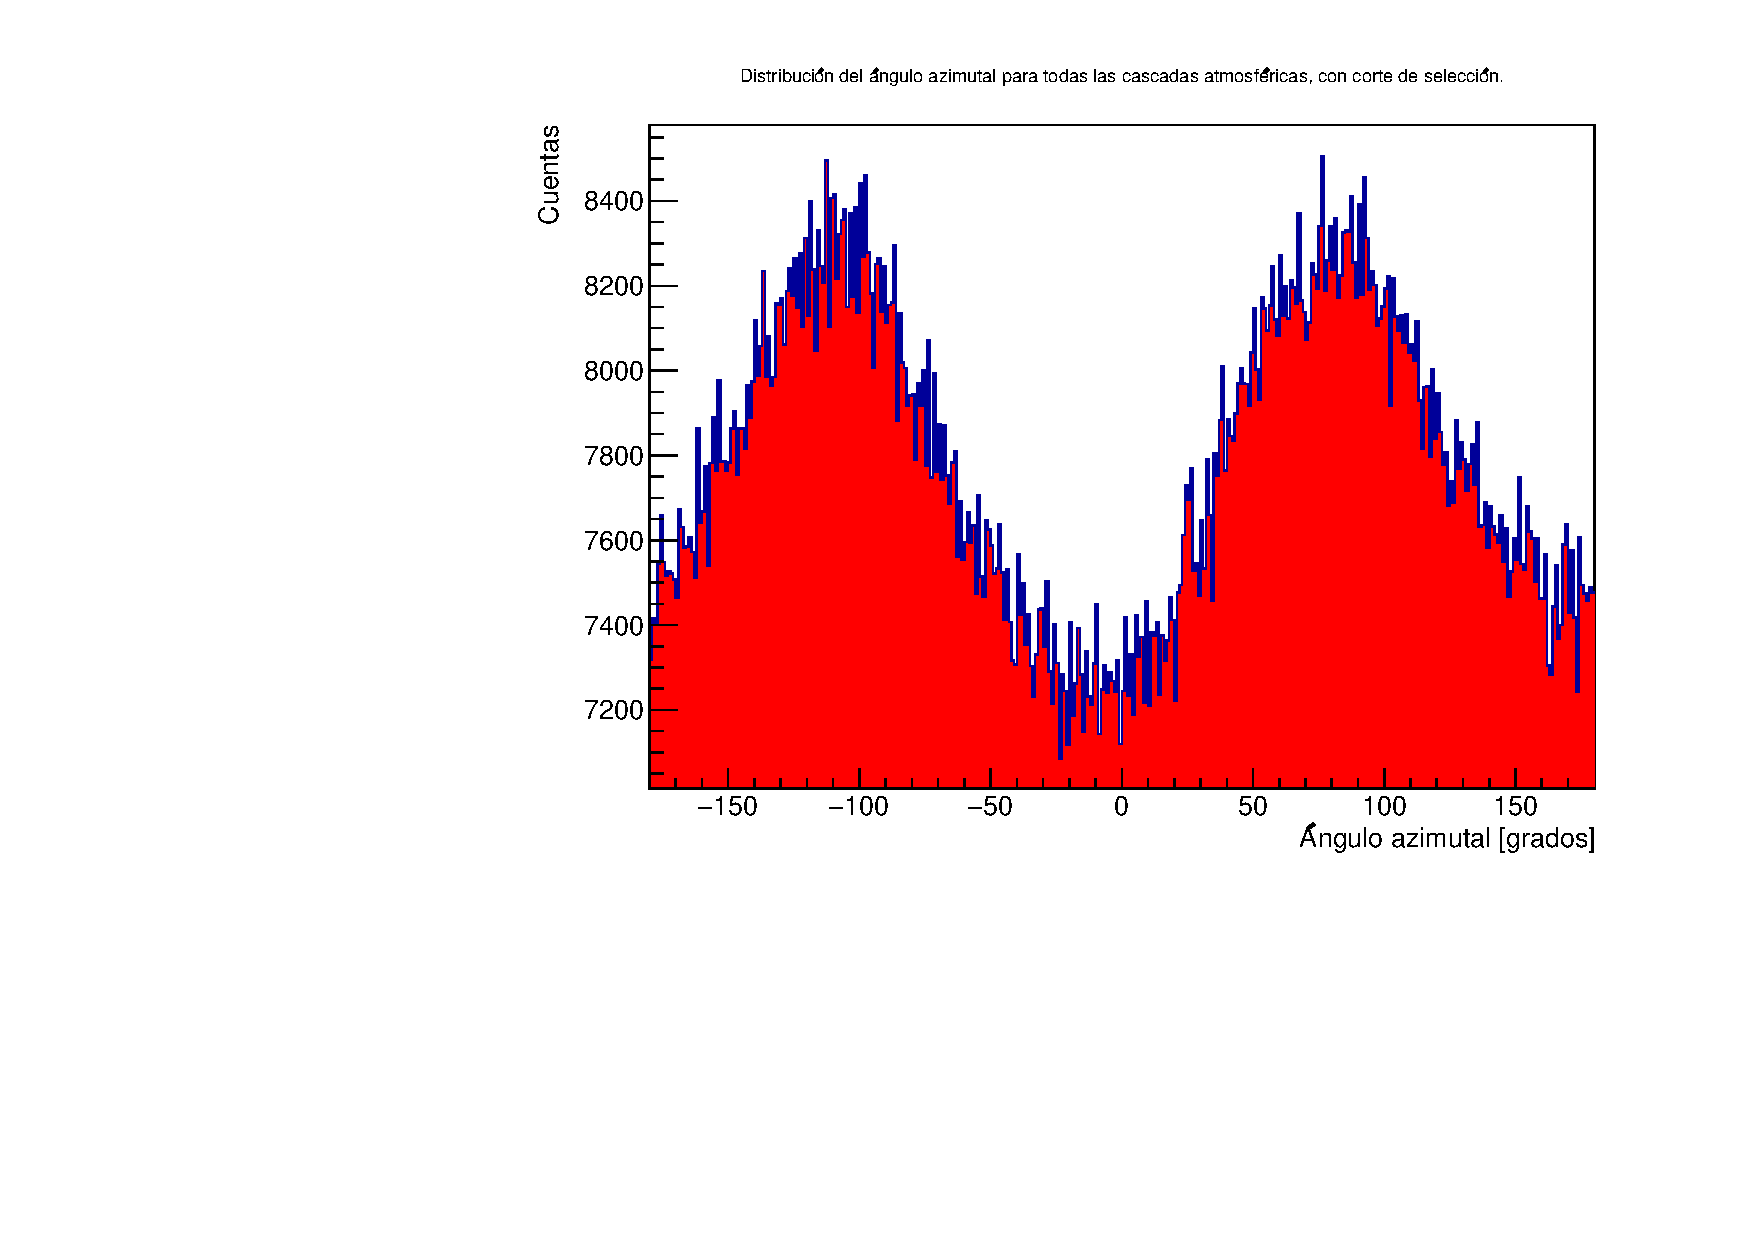
\includegraphics[width=0.9\textwidth]{../Figuras/Prob5B}
\caption{Distribución del ángulo azimutal para todos los eventos con corte de selección}
\label{fig:Prob5B}
\end{figure}



\end{document}